\documentclass[10pt]{report}
\usepackage[utf8]{inputenc}
\usepackage[greek,english]{babel}
\usepackage{alphabeta}
\usepackage{amsmath}
\usepackage{amssymb}
\usepackage{graphicx}
\usepackage{epstopdf}
\usepackage{inputenc}
\usepackage{geometry}
\usepackage{listings}
\usepackage{float}
\usepackage{xcolor}
\usepackage{titlesec}
\definecolor{codegreen}{rgb}{0,0.6,0}
\definecolor{codegray}{rgb}{0.5,0.5,0.5}
\definecolor{codepurple}{rgb}{0.58,0,0.82}
\definecolor{backcolour}{rgb}{0.95,0.95,0.92}
\definecolor{ceruleanblue}{rgb}{0.16, 0.32, 0.75}
\titleformat{\section}[block]{\color{ceruleanblue}\Large\bfseries\filcenter}{}{1em}{}
\titleformat{\subsection}[block]{\color{ceruleanblue}\Large\bfseries\filcenter}{}{0.5em}{}

\lstdefinestyle{mystyle}{
    backgroundcolor=\color{backcolour},   
    commentstyle=\color{codegreen},
    keywordstyle=\color{magenta},
    numberstyle=\tiny\color{codegray},
    stringstyle=\color{codepurple},
    basicstyle=\ttfamily\footnotesize,
    breakatwhitespace=false,         
    breaklines=true,                 
    captionpos=b,                    
    keepspaces=true,                 
    numbers=left,                    
    numbersep=5pt,                  
    showspaces=false,                
    showstringspaces=false,
    showtabs=false,                  
    tabsize=2
}

\lstset{style=mystyle}
\usepackage{hyperref}
\usepackage{lmodern}
\usepackage[T1]{fontenc}
\usepackage{textcomp}
\newcommand{\tu}{\textunderscore}
\usepackage{fancyhdr}
\geometry{left=2.5cm,right=2.5cm,top=2.5cm,bottom=2.5cm}
\pagestyle{fancy}
\fancyhf{}
\rhead{Φίλης Χάρης (ΑΕΜ: 9449)}
\chead{\href{https://github.com/harryfilis/Parallel_and_Distributed_Systems_Assignments/tree/master/KnnSearch}{KnnSearch-Repo-Link}}
\lhead{\emph{Distributed all-KnnSearch}}
\rfoot{Page \thepage}
\title{
KNN Search with MPI\\ 
\large Παράλληλα και Διανεμημένα Συστήματα\\ 
\textit{Assignment 2}}

\author{Φίλης Χάρης}
\date{\today}
\hypersetup{
    colorlinks=true,
    linkcolor=magenta,
    filecolor=magenta,      
    urlcolor=blue,
}
\graphicspath{ {./plots/} }
\begin{document}
\maketitle
\newpage
\begin{itemize}
\item Δείκτης στο αποθετήριο της εργασίας :\\
\href{https://github.com/harryfilis/Parallel_and_Distributed_Systems_Assignments/tree/master/KnnSearch}{https://github.com/harryfilis/Parallel-and-Distributed-Systems-Assignments/tree/master/KnnSearch}
\end{itemize}
\section{0 Το πρόβλημα  all-KnnSearch}
Στην παρούσα εργασία υλοποιείται ενας κατανεμημένος αλγόριθμος all-KNN search ο οποίος παραλληλοποιείται με την βοήθεια της διεπαφής MPI. Ο αλγόριθμος βρίσκει τους \textbf{k} κοντινότερους γείτονες(\emph{k-NN}) από κάθε σημείο ενός set \emph{X}.

Είσοδος του Αλγορίθμου είναι τα εξής:
\begin{itemize}
\item πινακας-set \textbf{X}
\item \textbf{n} πλήθος σημείων του πινακα Χ
\item \textbf{d} αριθμός διαστάσεων των σημείων
\item \textbf{k} αριθμός γειτώνων k για το οποίο θα γίνει το knnSearch
\end{itemize}
Κάθε MPI διαδικάσία \emph{Pi} θα υπολογίζει την απόσταση των δικών της σημείων από όλα τα άλλα σημεία και καταγράφει τις αποστάσεις(\textbf{distances || dmatrix || ndist}) και τους δείκτες του k πλησιέστερου για κάθε ένα από τα δικά του σημεία(αποθηκευση σε minarr στο searchVPT).


\section{1 v0.c Sequential - Ανάλυση αλγορίθμου}
Αρχικά Υλοποίηθηκε μια έκδοση του v0 σε matlab που παρατίθεται παρακάτω σε σχόλια εξηγείται η διαδικασία.
\href{https://github.com/harryfilis/Parallel-and-Distributed-Systems-Assignments/tree/master/KnnSearch/matlab/v0.m}{v0.m}

Οσον αφορά τον κώδικα σε c αυτος ακολουθεί το αρχείο matlab.
Αρχικά ορίζεται η δομή δεδομένων \textbf{knnresult} με τα εξής μελη :
\begin{itemize}
\item \textbf{*nidx} -> Indices (0-based) of nearest neighbors [m-by-k]
\item \textbf{double *ndist} -> Distance of nearest neighbors          [m-by-k]
\item \textbf{int n} -> Αριθμός των σημείων του ερωτήματος Υ
\item \textbf{int k} -> Αριθμός των k κοντινότερων γειτόνων
\end{itemize}

Στόχος να κρατήσουμε τα k κοντινότερα σημεία του Υ  στον X πινακα.
\subsection{1.1 Ανάλυση συνάρτησης \textbf{knnresult kNN(double *X, double *Y, int n, int m, int d, int k)} }
Αρχικά αρχικοποιοιείται κατάλληλα η επιστρεφόμενη δομή \emph{knnresult}.\footnote{(Το ndist εχει μεγεθος m*d doubles)}

Θέλουμε να υπολογίσουμε τον πίνακα διαστάσεων \textbf{distances} βάση του τύπου:

\begin{verbatim}
D = sqrt(sum(X.^2,2)- 2 *X*Y.' + sum(Y.^2,2).');
X matrix
Y.' transpose Y matrix
\end{verbatim}

\begin{enumerate}
\item Δεσμεύονται οι πίνακες xx,yy όπου υπολογίζοτναι και υλοποιούνται τα τετράγωνα των στοιχείων των πινάκων.
\item Ταυτόχρονα υπολογίζονται οι πίνακες \begin{verbatim}
y_sum,x_sum
\end{verbatim}οι οποίοι ειναι σε rowmajor format οπως ολοι οι 2d πίνακες.

\quad\item μεσω της βιβλιοθήκης cblas.h γίνεται η πραξη  - 2*X*Y' και αποθηκεύεται σε rowmajor format στον πινακα distances με την συνάρτηση \begin{verbatim}
 cblas_dgemm(CblasRowMajor, CblasNoTrans, CblasTrans, n, m, d, -2, X, d, Y, d, 0, distances, m);
\end{verbatim}
\item Στην συνέχεια αθροίζονται τα x\_sum και y\_sum στοιχεία στα στοιχεια του distances(για αυτό χρειάστηκε να είναι σε rowmajorformat)
\item Τώρα ο D matrix είναι έτοιμος και εκτελούμε quik\_select για να βρούμε τα k μικρότερα στοιχεία μέσω της kthSmallest(εδώ γίνεται μια πιο απλή υλοποίηση).
\item γινεται αποθηκευση των min distances στο knnresult.ndist σε row\_major και ομοίως και των indeces.
\item Επιστρέφεται η δομή knnresult result.
\end{enumerate}


\subsection{1.2 v0.c/main}
Εδώ αρχικά παίρνονται από τα command line arguments τα n,d,k,m για τυχαίο πείραμα και αρχικοποιείται η δομή knnresult(malloc,etc.)\\
Στην συνέχεια ορίζονται ψευδό τυχαίοι X, Y πίνακες με την βοηθεια της \textbf{randomBounded(double lower\_limit, double upper\_limit)}\\
Καλείται η kNN και μετράται ο χρόνος εκτέλεσης της.

\section{2 v1.c Asychronous - Ανάλυση Αλγορίθμου}
Γίνεται μια υλοποιηση σε matlab παλι \href{https://github.com/harryfilis/Parallel-and-Distributed-Systems-Assignments/tree/master/KnnSearch/matlab/v1.m}{v1.m}
Δεν χρησιμοποιώ την knnresult distrAllkNN(double * X int n, int d, int k); αλλά την συνάρτηση του  v0.c\\
Περνάω τα δεδομένα μεσω του MPI περιβάλλοντος σε ένα δαχτυλίδι οπου τσεκαρονται μεταξύ τους οι αποστάσεις και αλλάζει ο k\_nearest
\begin{figure}[h]
    \centering
   	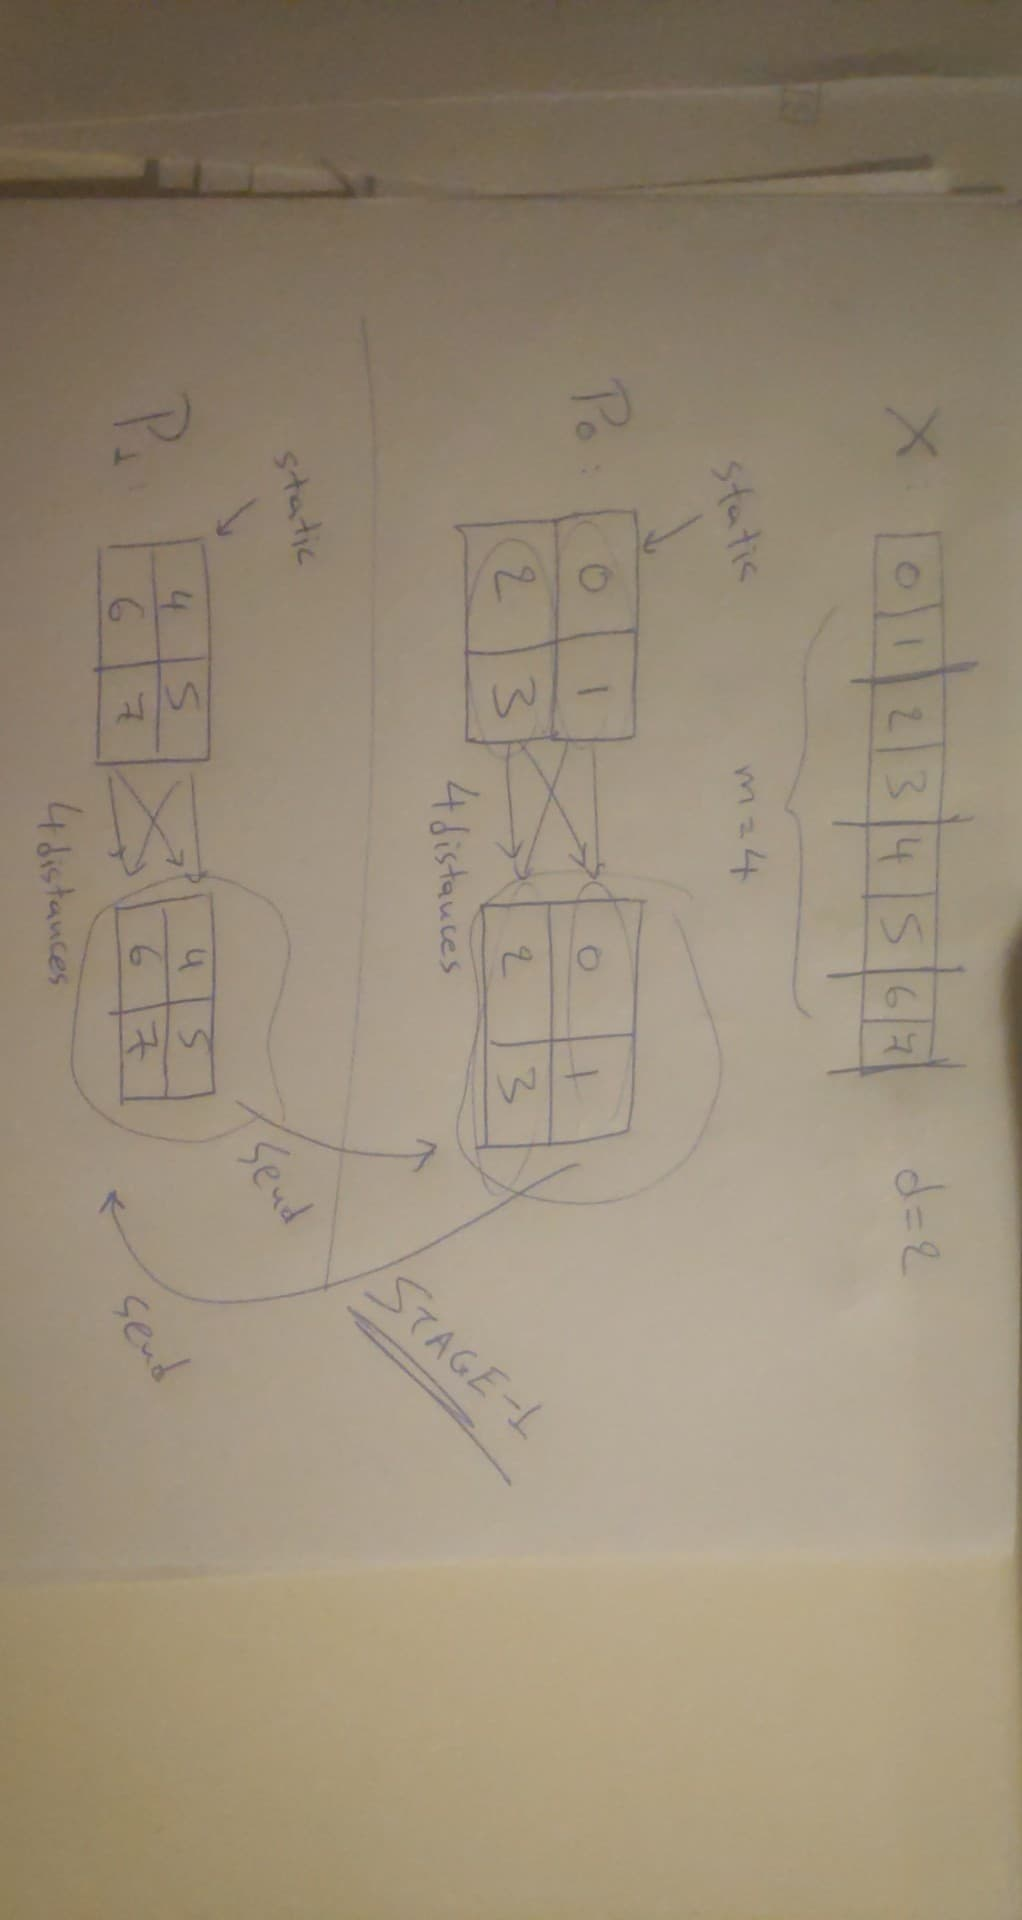
\includegraphics[scale=0.2,angle = 90]{../plots/ring.jpg}
    \caption{Ring\_Schematic}
    \label{fig:Ring\_Schematic}
\end{figure}\\
Q:\emph{How many times do we need to iterate to have all points checked against all other points?}\\
\\Ans: Every process has processed its own x\_i\_data, now they have to pass around data to each other in a ring mode
That has to repeat until each process has processed all possible data => p times\\

H αντιγράφή (memcpy)που γίνεται γίνεται σε θέσεις μνήμης.
*Αναλυτικά σχόλια υπάρχουν στον κώδικα στο πως διαχειρίζομαι τα processes και τα μηνυματα που στέλνω.

\section{3 v2.c Vantage Point tree - Ανάλυση αλγορίθμου}
Εδώ χρησιμοποιήθηκαν οι εξής ψευδοκώδικες σε matlab:
\lstinputlisting[language=Matlab]{../matlab/makeVPT.m}
\lstinputlisting[language=Matlab]{../matlab/searchVPT.m}
Οσον αφορά τον κώδικα σε c
Ορίζεται minArray struct που αποθηκεύονται απο κάθε  process τα οι μικρότερες απόστάσεις και οι δείκτες αυτών.
Oρίζεται επίσης η κλάση \textbf{node}  που είναι η βασική δομική μονάδα του vpTree.(εχει pointers σε left child και right child(τύπου node)).
\subsection{3.1 Συνάρτηση:node *vpTree\_create(double *x\_i\_data, node *root, int m, int d)}

Δημιουργεί ανδρομικά το δένδρο και επιστρέφει την ρίζα του.
Συγκεκριμένα:
\begin{enumerate}
\item Αρχικοποιεί τον πίνακα up του root με σημεία x\_i\_data(vp).
\item Υπολογίζει την μέση τιμή των αποστάσεων αυτών των σημείων της ρίζας
\item Aν οι αποστάσεις είναι μικρότερες απο την μέση τιμή της απόστασης των αποστάσεων της ρίζας τότε δημιουγείται αριστερό παιδί και αποθηκεύονται τα x\_i\_data σε row\_major format εκεί.
\item Aλλιώς γίνεται δεξί παιδί κτλ.
\item Τέλος καλείται η vpTree\_create για το αριστερό και το δεξί παιδί και αναδρομικά δημιουργείται το δένδρο.
\item επιστρέφεται το root.

\end{enumerate}

\subsection{3.2 Συνάρτηση:void searchVPT(double *x\_query, node *root, int d, int k, minArray* min\_arr)}
Αναδρομική συνάρτηση που αρχικά υπολογίζει την απόσταση των  x\_query από το vantage point του root και τα αποθηκεύει στον min\_arr.
Η radius παίρνει την απόσταση του γείτονα  k.Αν η απόσταση είναι μικρότερη απο την μέση τιμή των αποστάσεων της τωρινής ρίζας + της radius καλείται η searchVPT για το ίδιο x\_query αλλά με root το αριστερό παιδί της root και αυτό κάνει την αναδρομή.Αντίθετα η αναδρομή γίνεται για το δεξι υποδένδρο μέχρι και στις δύο περιπτώσεις να φτάσουμε σε φύλλο.

Η αναδρομή τελειώνει αν root == NULL δηλαδή το προηγούμενο root είναι φύλλο(τερματικός κόμβος). 

Η main χρησιμοποιεί MPI και έχει αναλυτικά σχόλια για την κατανόηση και το πώς στο s\_knn\_result αποθηκεύονται εν τέλει οι \emph{kNN}.


\section{Διαγράμματα και Προβλήματα}

\subsubsection{Προβλήματα}
\begin{enumerate}
\item Όταν έφτιαξα τρόπο να διαβάζω τους πίνακες που μας δώσατε πετούσε segmentation fault και δεν κατάφερα να τρέξω κανονικά για τους πίνακες παρόλο που έχω έτοιμα \textbf{ShellScripts} για το slurm που τρέχουν όλους τους πίνακες και κατέθεσα στην υπολογιστική μονάδα batches.(το λέω για να είμαι ειλικρινής.)
\item Η υπολογιστική μοναδα δεν ηταν προσβάσιμη λόγω του οτι δεν μας έδινε access στο vpn και επίσης είχαν κατατεθεί πολλές εργασίες όποτε η δικιά μου δεν προλαβε να ολοκληρωθεί.
\end{enumerate}
\subsubsection{Διαγράμματα}
Έγιναν 4 διαγράμματα από αρχικά batches που είχα θέσει στο hpc για τυχαίους πίνακες.

\begin{figure}[H]
\centering
\left.
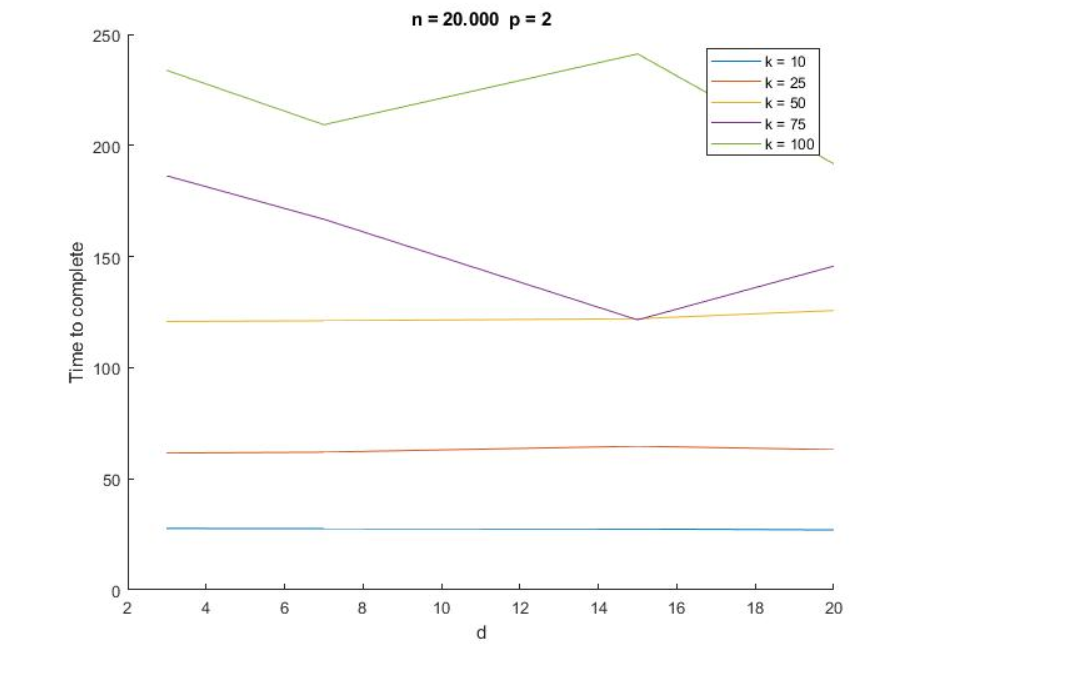
\includegraphics[scale=0.4]{../plots/v1_diagram_Random_array_.png}
\caption{./v1 n=20.000 p = 2}
\end{figure} 
\begin{figure}[H]
\centering
\left.
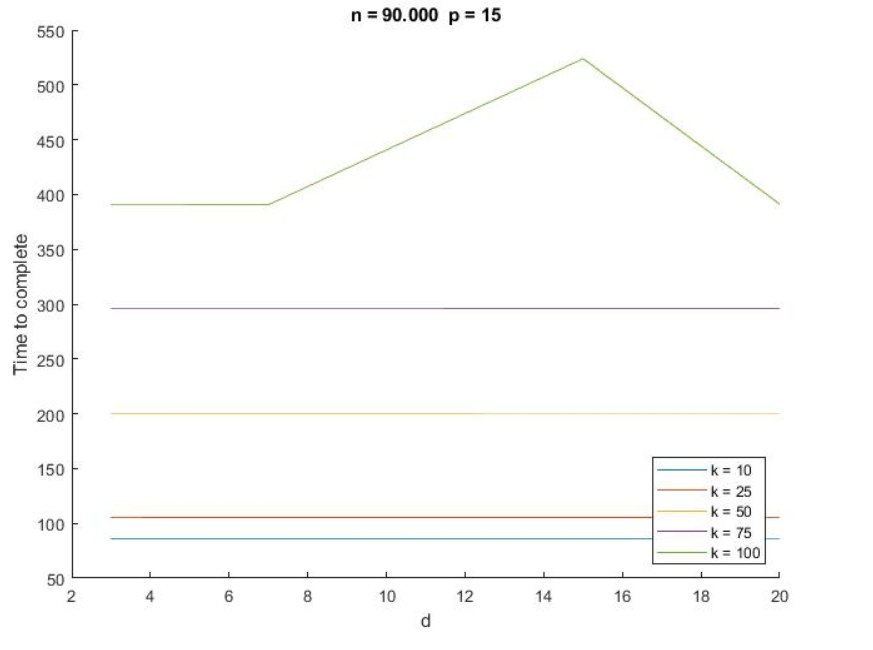
\includegraphics[scale=0.4]{../plots/v1_diagram_Random_array_2.png}
\caption{./v1 n=90.000 p = 15}
\end{figure} 
\begin{figure}[H]
\centering
\left.
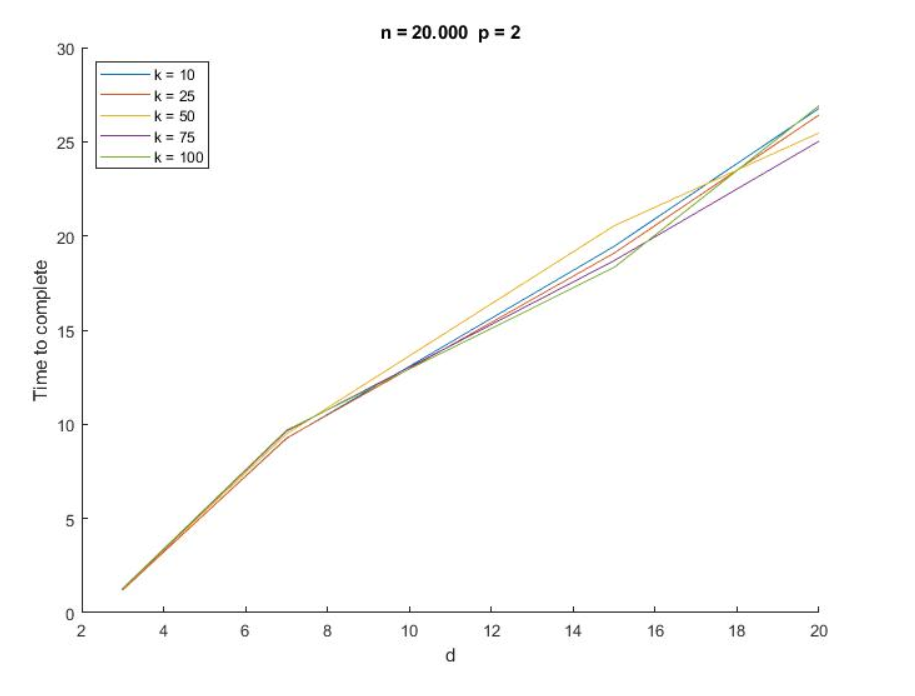
\includegraphics[scale=0.4]{../plots/v2_diagram_Random_array_.png}
\caption{./v2 n=20.000 p = 2}
\end{figure} 
\begin{figure}[H]
\centering
\left.
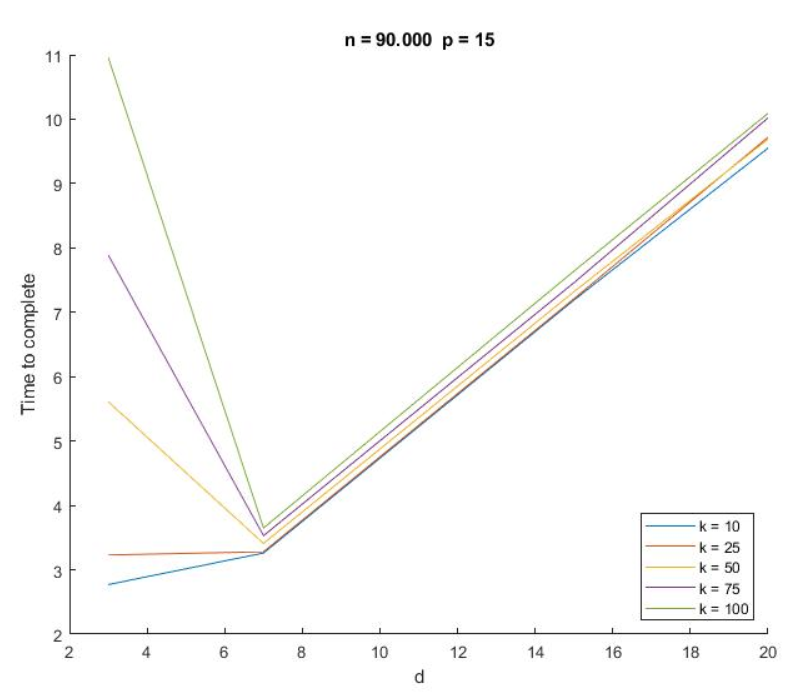
\includegraphics[scale=0.4]{../plots/v2_diagram_Random_array_2.png}
\caption{./v2 n=90.000 p = 15}
\end{figure} 

\subsubsection{Παρατηρήσεις}
Βλέπουμε σαφή βελτίωση με την χρήση του vpTree.

\subsubsection{ΤΕΛΟΣ ΑΝΑΦΟΡΑΣ}


\end{document}